\cotefile{29}
\scanpage{102}
\mspage{101}
\margin{\figure{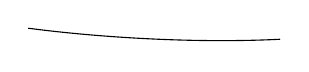
\begin{tikzpicture}\draw (0,0) .. controls (1,-.13) and (2.2,-.19) .. (3.2,-.14);\end{tikzpicture}}}

Examinons maintenant le cas où l'un des cycles $\underline{a}$ ou $\underline{b}$ (par exemple $\underline{b}$) appartient au noyau d'Albanese $Z_{\handwritten{\ell}}(A)$ ; par linéarité, on se ramène au cas où $\underline{b}$ est de la forme $\underline{c}_u-\underline{c}$, avec $\underline{c}\handwritten{\in}Z^{s}_{\unsure{o|0}}(A)_{\bar{\underline{k}}}$, et $u\handwritten{\in}{}^{s}A_{\bar{\underline{k}}}$. D'après l'invariance du symbole $j_{\handwritten{o}}$ par la translation $\handwritten{\tau_u}$, les deux membres de (3) sont respectivement égaux à $j_{\handwritten{o}}(Y_{\underline{a}},\underline{c})$ et à $j_{\handwritten{o}}(Y^{-}_{\underline{c}},\underline{a})$\handwritten{, en} \inserted{\handwritten{posant $Y=X_u-X$.}} Puisqu'on a $X\handwritten{\in}D_a(A)$, on a $Y\handwritten{\sim}0$, et on est ramené au cas déjà traité.

Supposons maintenant $X$, $\underline{a}$ et $\underline{b}$ quelconques. On peut, en modifiant $\underline{b}$ par l'addition d'un élément de $Z^{\handwritten{s}}_{\handwritten{\ell}}(A)_{\handwritten{\bar{\underline{k}}}}$, se ramener au cas où le cycle $\underline{a}^{-}\handwritten{\otimes}\underline{b}$ est étranger à $X$. Les symboles $X_{\underline{a}}(\underline{b})$ et $X^{-}_{\underline{b}}(\underline{a})$ sont alors définis, et on a
\[
X_{\underline{a}}(\underline{b})=X^{-}_{\underline{b}}(\underline{a}),\quad\text{d'où}\quad v(X_{\underline{a}}(\underline{b}))=v(X^{-}_{\underline{b}}(\underline{a})).
\]

D'autre part, soit $a$ (resp. $b$) l'un quelconque des composants de $\underline{a}$ (resp. $\underline{b}$). Alors les symboles $i(X_a,b)$ et $i(X^{-}_b,a)$ sont définis ; l'application $\handwritten{\unsure{\zeta|\xi}}:A\handwritten{\longrightarrow}A$ définie par $\handwritten{\zeta}(x)=a+b-x$ étant \uline{p}-isomorphique en $b^{\handwritten{\unsure{\circ|o|0}}}$, de valeur $a^{\handwritten{\circ}}$, on a, d'après la propriété d'invariance du symbole $i$,
\[
i(X_a,b)=i(X^{-}_b,a).
\]

Il en résulte, par linéarité,
\margin{\figure{\begin{tikzpicture}\draw (0,0)--(.02,-.22);\end{tikzpicture}}}
\[
i(X_{\underline{a}},\underline{b})=i(X^{-}_{\underline{b}},\underline{a}).
\]

Compte tenu des formules (2) précédentes, on en déduit (3).

Notons enfin que $j_{\handwritten{o}}(X,\underline{a})$ s'annule lorsque tous les composants de $A$ appartiennent au groupe ${}^{s}A_{\bar{\underline{k}},\handwritten{o}}$. En effet, soit $f$ une fonction sur $V$, définie sur $\underline{k}$, telle que

% archive sheet number: 101
\scanpage{113}

\uline{Théorème de Bertini et variantes}.

Dans la suite $k$ désigne un corps, $P^r=P^r_k$.

\margin{\figure{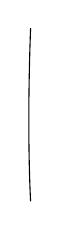
\begin{tikzpicture}\draw (0,0) .. controls (-.03,-.8) and (-.03,-1.6) .. (0,-2.2);\end{tikzpicture}}}
\uline{Théorème de Bertini} 1: Soit $f:X\handwritten{\rightarrow}P^r_k$ un morphisme, où $X$ est un schéma algébrique géométriquement irréductible, et soit $n=\dim\overset{\handwritten{\rule{1.9em}{.4pt}}}{f(X)}$. Soit $L_t$ le\deleted{\unsure{s|un}} sous-espace linéaire de codimension $s$ \uline{générique} de $P^r$, où $s$ est un entier fixé $\handwritten{\leq}n-1$. Alors $\inserted{Y_t=}f_t^{-1}(L_t)\handwritten{\subset}X_t=X\otimes_k k(t)$ est géométriquement irréductible.

\margin{\handwritten{\unsure{prouvé|repris} dans SGA \unsure{V|IV}}\figure{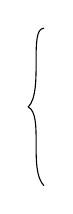
\begin{tikzpicture}\draw (.2,0) .. controls (0,0) and (.2,-.8) .. (0,-1) .. controls (.2,-1.1) and (0,-1.8) .. (.2,-2);\end{tikzpicture}}}
\margin{\figure{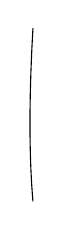
\begin{tikzpicture}\draw (0,0) .. controls (-.04,-.7) and (-.06,-1.5) .. (0,-2.2);\end{tikzpicture}}}
\inserted{\uline{Enoncé local} 2: Soit $f:X\handwritten{\rightarrow}P^r$ un morphisme, avec $X$ un schéma algébrique.} \deleted{\uline{\unsure{Complément:}} \unsure{Supposons}} Soit $Z\handwritten{\rightarrow}X$ \deleted{\illegible{2}} l'ensemble des points de $X$ en lesquels \inserted{\handwritten{soit}} $f$ est \deleted{\handwritten{\unsure{soit|non}}} ramifié \deleted{ou en lesquels} \inserted{\handwritten{soit}} $X$ n'est pas géométriquement unibranche (resp.\ \inserted{\handwritten{pas}} normal, resp.\ \inserted{\handwritten{pas}} lisse \ldots), \deleted{alors} et supposons que $\overset{\handwritten{\rule{1.9em}{.4pt}}}{f(Z)}$ soit de dimension $\handwritten{<}s$. Alors $\inserted{Y_t=}f_t^{-1}(L_t)$ est géométriquement unibranche (resp.\ normal, resp.\ lisse \ldots), où $L_t$ est comme ci-dessus.

De ces deux énoncés on déduit\handwritten{/}formellement;

\margin{\figure{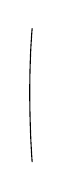
\begin{tikzpicture}\draw (0,0) .. controls (-.05,-.6) and (-.03,-1.3) .. (0,-1.7);\end{tikzpicture}}}
\deleted{\unsure{Th|Thé}}\uline{Corollaire} 3: Soit $f:X\handwritten{\longrightarrow}P^r$ satisfaisant les conditions de 1\handwritten{,} et 2 non respé.\ \inserted{Supposons $k$ alg.\ clos.} Alors le\deleted{inclusion} morphisme canonique
\[
\handwritten{\pi}_1(Y_{\bar{t}})\handwritten{\rightarrow}\handwritten{\pi}_1(X)
\]
est surjectif.

\uline{\unsure{Remarque}} \unsure{\deleted{4}3|\deleted{3}4}. Utilisant les théorèmes de changement de base pour le $\handwritten{\pi}_1$, on conclut \deleted{que} (posant $X_{\bar{t}}=X\otimes_k k(\bar{t})$) que l'homomorphisme $\deleted{\unsure{\pi}_1}$
\[
\handwritten{\pi}_1(Y_{\bar{t}})\handwritten{\rightarrow}\handwritten{\pi}_1(X_{\bar{t}})\tag*{(*)}
\]
est surjectif si $X_{\deleted{\unsure{t|\bar{t}}}}$ est propre, et que l'homomorphisme
\[
\handwritten{\pi}_1^{!}(\unsure{\deleted{Y}X|\deleted{X}Y}_{\bar{t}})\handwritten{\rightarrow}\handwritten{\pi}_1^{!}(X_{\bar{t}})\tag*{\handwritten{(**)}}
\]
est surjectif, où le ! désigne le plus grand quotient profini premier à l'è\unsure{\deleted{d}x|\deleted{x}d}posant car.\ de $k$. On n'affirme pas, cependant, que (*) soit toujours surjectif (sans hypothèse de propreté sur $X$).

On déduit, de 1, par une application facile du théorème de connexité:

\margin{\handwritten{\unsure{vu.|vu} dans SGA V}\figure{\begin{tikzpicture}\draw (0,0)--(.03,-.5);\end{tikzpicture}}}
\uline{Corollaire} 4 (de 1): Sous les conditions de 1) pour $f:X\handwritten{\longrightarrow}P^r$, si $X$
% archive sheet number: 112
\scanpage{114}
\margin{\figure{\begin{tikzpicture}\draw (0,0)--(.02,-.8);\end{tikzpicture}}}
est de plus propre, alors pour \uline{toute} sous-variété linéaire $\inserted{L_t}$ de codimensio\handwritten{n} $s$, $Y_t=f_t^{-1}(L_t)$ est géométriquement connexe.

Conjuguant avec 2, on trouve, par l'argument qui a permis de déduire 3 de 1 :

\margin{\handwritten{cf. SGA 1 X \unsure{2.11|2,11|2.II}}}
\margin{\figure{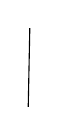
\begin{tikzpicture}\draw (.02,0)--(0,-1);\end{tikzpicture}}}
\uline{Corollaire} 5: \deleted{Avec}\inserted{\handwritten{Sous}} les hypothèses de \unsure{\deleted{4}3|\deleted{3}4}, \inserted{avec $X$ propre,} l'homomorphisme danonique $\handwritten{\pi}_1(Y_{\bar{t}})\handwritten{\rightarrow}\handwritten{\pi}_1(X)$ ($\handwritten{\simeq}\handwritten{\pi}_1(X_{\bar{t}})$ par le théorème de changement de base) est surjectif.

Nous désirons également un énoncé analogue à 5, donnant une surjectivité pour des $\handwritten{\pi}_1$ pour un $t$ non générique, mais sans hypothèse de propreté, et pour des quotients plus gros du $\handwritten{\pi}_1$ que ceux envisagés dans (**). On peut\deleted{\unsure{on|nt}} donner à ce sujet le résultat suivant:

\margin{\figure{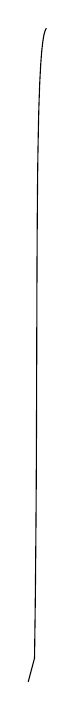
\begin{tikzpicture}\draw (.15,0) .. controls (-.02,-.2) and (.06,-4) .. (0,-8) --(-.08,-8.3);\end{tikzpicture}}}
\uline{Théorème} 6. \unsure{Supposons|Suipposons} $k$ algébriquement clos, \inserted{\handwritten{et}} $X$ propre, $f:X\handwritten{\rightarrow}P^r$, \deleted{et} le sous -espace linéaire $L_t$ de $P^r$ de codimension $s$ (défini sur $k$, pour fixer les idées) \deleted{tels qu'on ait} et enfin le sous-schéma fermé $D$ de $X$ tels qu'on ait ceci; \deleted{où on a posé $U=X-D$}

a) \deleted{$\unsure{U}_t=\unsure{U}\unsure{\cap}X_t$ et} $\deleted{X}\handwritten{Y}_t=f^{-1}(L_t)$ est non vide.

b) Pour tout $x\handwritten{\in}\deleted{X}\handwritten{Y}_t$, $X$ est lisse en $x$, $Y_t$ est lisse en $x$\handwritten{,} de codi\unsure{\deleted{mem}men|\deleted{men}mem}sion $s$ dans $X$ en $x$, $f$ est net en $x$.

c) Pour tout $x\handwritten{\in}D_t=D\handwritten{\cap}Y_t$, o\deleted{\`{}}u \deleted{bien} bien $\operatorname{codim}_x(D_t,\deleted{\unsure{X|T}}\handwritten{Y}_t)\handwritten{\geq}2$, ou bien $D_{\deleted{\unsure{t}}}$ est un diviseur \unsure{enr|sur} $X$ en $x$ et $\deleted{D_t}$ induit sur $Y_t$ en $x$ un diviseur à croisements normaux.

\unsure{Supposons|Suipposons} $U=X-D$ irréductible, et considérons l'inclusion $U_t=U\handwritten{\cap}Y_t\handwritten{\longrightarrow}U$. \deleted{Alors $\unsure{U|Y}_t$} Soit $\handwritten{\pi}_1^t(U)$ le \deleted{\unsure{grou|gros}} quotient du groupe fondamental de $U$ \deleted{formé des} qui classifie les revêtements de $U$ qui sont modérément ramifiés en les composantes irréductibles de codimension 1 de $D$ dans $X$ qui rencontrent $Y_t$, \deleted{(\unsure{i.e.} telles que $D$} et $\handwritten{\pi}_1^t(\unsure{\mathbb{U}|\deleted{V}U|\deleted{U}V|\mathbb{V}}_t)$ le quotient \deleted{analogue} de $\handwritten{\pi}_1(U_t)$ qui classifie les revêtements qui sont modérément ramifiés en les composantes irréductibles de codimension 1 de $D_t$. On a un homomor%
% archive sheet number: 113
\scanpage{115}%
phisme évident
\margin{\figure{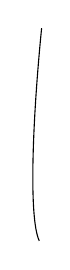
\begin{tikzpicture}\draw (.03,0) .. controls (-.08,-1.1) and (-.14,-2.4) .. (0,-2.7);\end{tikzpicture}}}
\[
\handwritten{\pi}_1^t(U_t)\handwritten{\rightarrow}\handwritten{\pi}_1^t(U)
\]
(un point-base géométrique de $U_t$ étant choisi). Cet homomorphisme est \uline{surjectif}.

Démonstration. Lorsqu'on remplace $L_t$ par $L_{t'}$ générique, alors la conclusion est contenue dans le corollaire 3, en d'autres termes, si $\unsure{\mathbb{U}|\deleted{V}U|\deleted{U}V|\mathbb{V}}$ est un revêtement étale \inserted{connexe} de $U$ \deleted{\unsure{tel que sa}} (satisfaisant la condition de modération en\unsure{\deleted{g}v|g}isagée - en fait, ce n'est pas nécessaire, enx vertu de 3 ) alors sa restriction $V_{t'}$ au dessus de $U_{t'}$ est connexe. On veut prouver que sa restriction $V_t$ au dessus de $U_t$ est \inserted{\handwritten{également}} connexe. Or pour un paramètre variable sur \inserted{\handwritten{un voisinage ouvert assez petit $T$ de}} la grassmanienne $\deleted{\unsure{T|G}}$ des $L_{t'}$\handwritten{,} \deleted{et voisin de $t$, la famill\unsure{e}} \inserted{\handwritten{la}} famille des $Y_{t'}$ est un morphisme propre et lisse $Y\handwritten{\rightarrow}T$, et celle des $D_{t'}$ est un sous-schéma fermé \deleted{de} $\handwritten{\Delta}$ de $Y$, qui est la réunion d'un sous-schéma $\handwritten{\Delta}_1$ qui est de codi\unsure{\deleted{mem}men|\deleted{men}mem}sion $\handwritten{\geq}2$ sur chaque fibre (et qui ne comp\unsure{\deleted{t}|t}e\inserted{\handwritten{\unsure{m|nt|n}}} pas, à cause du théorème de pureté relative) et d'un diviseur $\handwritten{\Delta_2}$ à croise\`{m}ents normaux relatifs. Le revêtement donné $V$ de $U$ définit un revêtement \deleted{$V$ de $Y$} $V'$ de $U'=Y-\handwritten{\Delta}$, et il\deleted{\unsure{f|x}} faut montrer que la restriction de celui-ci à la fibre géométrique de $t$ est connexe, sachant qu'il en est ainsi de sa restriction à la fibre géométrique en $t'$, la générisation maximale de $t$. Or par la pureté, on sait que $V'$ se prolonge en un revêtement étale $V''$ de $U''=Y-\handwritten{\Delta_2}$, et par hypothèse ce dernier est modérément ramifié sur les fibres, relativement au diviseur $\handwritten{\Delta_2}$. La conclusion est alors une conséquence du théorème \deleted{\unsure{connu}} de spécialisation pour le groupe fondamental modéré, qui figure(ra) dans SGA 1 XIII (exposé de Mme Raynaud).

\uline{Remarque}7.Avec les notations de SGA 7 XVIII\handwritten{,} 6 s'applique pour tout pinceau de Lefschetz $D$ pour fournir la surjectivité de\deleted{s quotients par}
% archive sheet number: 114
\scanpage{116}
l'homomorphisme $\handwritten{\pi}_1^t(D-\overset{\handwritten{\scriptscriptstyle\vee}}{D})\handwritten{\rightarrow}\handwritten{\pi}_1^t(\unsure{\mathbb{P}|\deleted{R}P}-\overset{\handwritten{\scriptscriptstyle\vee}}{X})$, et donne le théorème de conjugaison des cycles évanescents (donc le théorème d'irréductibilité de la cohomologie évanescente) pourvu qu'on ne soit pas dans le cas $\operatorname{car}.k=2$ et $\dim X$ impaire (NB \deleted{ce n'est pas,} dans la situation du th. de Griffiths, il n'y a donc pas d'ennui). Dans ce dernier cas, par contre, je ne sais \deleted{rien} pas prouver\inserted{la conjuga\unsure{\deleted{n}i|i}son sous $\handwritten{\pi}_1(D-\overset{\handwritten{\scriptscriptstyle\vee}}{D})$}, sauf pour un pinceau \uline{générique}, puisqu'alors la représentation envisagée est sauvage; \inserted{j'ignore si \unsure{ella|elle|\deleted{cela}\handwritten{elle}} reste vrai\handwritten{\unsure{e}} pour un pinceau \uline{général}.} Noter cependant que la conjugaison des sous-groupes de monodromie locale\deleted{\unsure{,|s}} \uline{dans} $\operatorname{Aut}(H^{n-1}\handwritten{(Y_{\bar{\eta}}))}$ (qui est très élémentaire) reste vraie, bien entendu, et celle-ci suffit pour prouver le théorème que j'ai proposé (au par. 6 de XVIII) caractérisant le cas où la condition (A) n'est \uline{pas} vérifiée.
% archive sheet number: 115
